 \documentclass{standalone}
 \usepackage{tikz}
 \usepackage{pgfplots}
 \pgfplotsset{width=10cm,compat=1.9}
\newcommand{\bA}{{\mathbf{A}}}
 \begin{document}

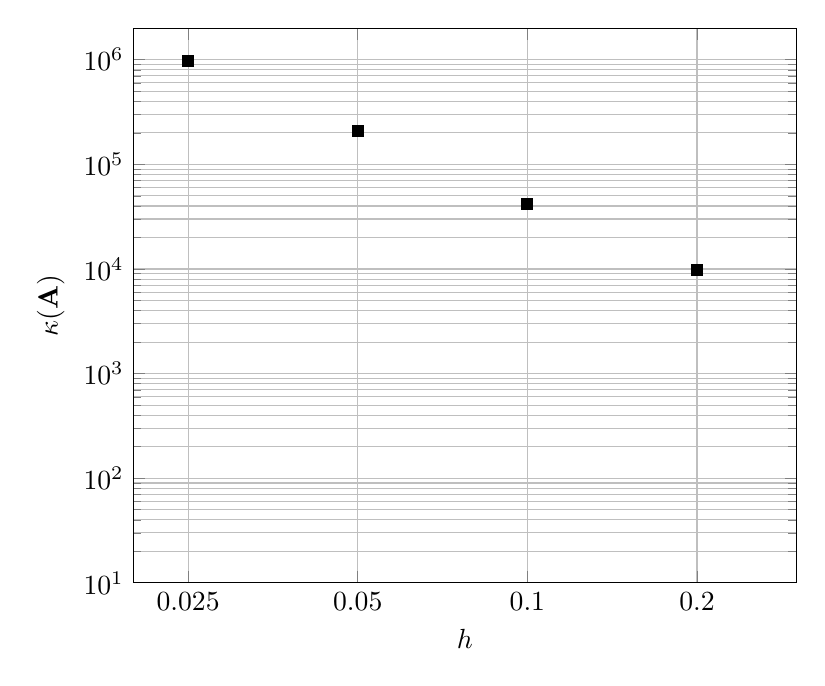
\begin{tikzpicture}
\begin{axis}[
xmin=0.02, xmax=0.3, ymin = 1.0E1, ymax = 2.0E6,
xlabel={$h$}, ylabel={$\kappa(\bA)$}, 
xmode=log,ymode=log,grid=both,scatter/classes=
{a={mark=*,black},
b={mark=square*,black}},
xtick={0.025,0.05,0.1,0.2},
xticklabels={$0.025$,$0.05$,$0.1$,$0.2$}
]
\addplot[scatter, only marks,scatter src=explicit symbolic
]
table[col sep=comma,meta=label]{
x,y,label
%0.2,2.22e1,a
%0.1,2.47e1,a
%0.05,2.71e1,a
%0.025,2.95e1,a
0.2,9.8e3,b
0.1,4.2e4,b
0.05,2.1e5,b
0.025,9.8e5,b
};
\end{axis}
\end{tikzpicture}
\end{document}
